%%%%%%%%%%%%%%%%%%%%%%%%%%%%%%%%%%%%%%%%%%%%%%%%%%%%%%%%%%%%%%%%%%%%%%%%
% Uni Duesseldorf
% Lehrstuhl fuer Datenbanken und Informationssysteme
% Vorlage fuer Bachelor-/Masterarbeiten
% Optimiert fuer den Original-Latex-Kompiler LATEX.EXE (LaTeX=>PS=>PDF)
%%%%%%%%%%%%%%%%%%%%%%%%%%%%%%%%%%%%%%%%%%%%%%%%%%%%%%%%%%%%%%%%%%%%%%%%
% Ueberarbeitung für pdflatex (LaTeX=>PDF)
%%%%%%%%%%%%%%%%%%%%%%%%%%%%%%%%%%%%%%%%%%%%%%%%%%%%%%%%%%%%%%%%%%%%%%%%
% Vorlage Changelog:
% 10.09.2015 (Matthias Liebeck): Nummerierung des Inhaltsverzeichnis nun römisch, Beispiel für einen Anhang eingebaut, \raggedbottom hinter sections eingefügt
% 11.07.2018 (Matthias Liebeck): Ersetzung des Bibliographiestils, Einsatz von Biber
% 04.09.2018 (Matthias Liebeck):
%   * Bibtex: unnötige Bibtexfelder beim Rendern ausblenden (thx @ Markus Brenneis)
%   * ngerman: "et al." im BibTeX für drei oder mehr Autoren
%   * Neuer Befehl \sectionforcestartright: Sections immer rechts beginnen (thx @ Philipp Grawe)
%   * ngerman: Deutsche Anführungszeichen im Literaturverzeichnis (thx @ Markus Brenneis)
%   * ngerman: Deutsche Anführungszeichen im Literaturverzeichnis (thx @ Markus Brenneis)
% 16.10.2018 (Matthias Liebeck): Zwei fixes an \sectionforcestartright (thx @ Markus Brenneis)
%%%%%%%%%%%%%%%%%%%%%%%%%%%%%%%%%%%%%%%%%%%%%%%%%%%%%%%%%%%%%%%%%%%%%%%%
%%%% BEGINN EINSTELLUNG FUER DIE ARBEIT. UNBEDINGT ERFORDERLICH! %%%%%%%
%%%%%%%%%%%%%%%%%%%%%%%%%%%%%%%%%%%%%%%%%%%%%%%%%%%%%%%%%%%%%%%%%%%%%%%%
% Geben Sie Ihren Namen hier an:

\newcommand{\bearbeiter}{Robin Kösters}

% Geben Sie hier den Titel Ihrer Arbeit an:
\newcommand{\titel}{Klassifikation von Tweets zur Erkennung von Trollen}

% Geben Sie das Datum des Beginns und Ende der Bachelorarbeit ein:
\newcommand{\beginndatum}{18. September 2020}
\newcommand{\abgabedatum}{18.~Dezember~2020}

% Geben Sie die Namen des Erst- und Zweitgutachters an:
\newcommand{\erstgutachter}{Prof. Dr.~Stefan Conrad}
\newcommand{\zweitgutachter}{Prof. Dr.~Martin Mauve}

% Falls Sie die Arbeit zweiseitig ausdrucken wollen,
% benutzen Sie die folgende Zeile mit
% \AN fuer zweiseitigen Druck
% \AUS fuer einseitigen Druck
\newcommand{\zweiseitig}{\AN}
% true fuer biber, false fuer klassischen Zitierstil
%\newcommand{\biber}{false}
\newcommand{\biber}{true}

% Falls Sections immer rechts beginnen sollen. Gerade für Masterarbeiten
% interessant. Bei kurzen Bachelorarbeiten eher weniger zu verwenden.
\newcommand{\sectionforcestartright}{false}
%\newcommand{\sectionforcestartright}{true}

% Falls die Arbeit in englischer Sprache verfasst
% werden soll, dann benutzen Sie die folgende Zeile mit
% englisch fuer englische Sprache
% deutsch fuer deutsche Sprache
\newcommand{\sprache}{deutsch}

% Hier wird eingestellt, ob es sich bei der Arbeit um eine Bachelor-
% oder Masterarbeit handelt (unpassendes auskommentieren!):
\newcommand{\arbeit}{Bachelorarbeit}
%~ \newcommand{\arbeit}{Masterarbeit}


%%%%%%%%%%%%%%%%%%%%%%%%%%%%%%%%%%%%%%%%%%%%%%%%%%%%%%%%%%%%%%%%%%%%%%%%
%%%% ENDE EINSTELLUNGEN %%%%%%%%%%%%%%%%%%%%%%%%%%%%%%%%%%%%%%%%%%%%%%%%
%%%%%%%%%%%%%%%%%%%%%%%%%%%%%%%%%%%%%%%%%%%%%%%%%%%%%%%%%%%%%%%%%%%%%%%%

% Die folgende Zeile NICHT EDITIEREN oder loeschen


%%%%%%%%%%%%%%%%%%%%%%%%%%%%%%%%%%%%%%%%%%%%%%%%%%%%%%%%%%%
% Obere Titelmakros. Editieren Sie diese Datei nur, wenn
% Sie sich ABSOLUT sicher sind, was Sie da tun!!!
% (Z.B. zum Abaendern der BA-Vorlage in eine MA-Vorlage)
% Uni Duesseldorf
% Lehrstuhl fuer Datenbanken und Informationssysteme
% Version 2.2 - 2.3.2010
%%%%%%%%%%%%%%%%%%%%%%%%%%%%%%%%%%%%%%%%%%%%%%%%%%%%%%%%%%%
\newcommand{\AN}{twoside}
\newcommand{\AUS}{}


%\newcommand{\englisch}{}
%\newcommand{\deutsch}{\usepackage[german]{babel}}

%% Die folgenden auskommentierten Optionen dienen der automatischen
%% Erkennung des Latex-Kompilers und dem Setzen der davon abhängigen
%% Einstellungen. Bei Problem z.B. mit dem Einbinden von verschiedenen
%% Grafiktypen bei Verwendung von PdfLatex oder Latex, einfach die
%% verschiedenen \usepackage(s) ausprobieren. (Mit diesen Einstellungen
%% funktionierte diese Vorlage bei der Verwenundg von latex.exe als
%% Kompiler bei den meisten Studierenden.)

%\newif\ifpdf \ifx\pdfoutput\undefined
%\pdffalse % we are not running pdflatex
%\else
%\pdfoutput=1 % we are running pdflatex
%\pdfcompresslevel=9 % compression level for text and image;
%\pdftrue \fi

\documentclass[11pt,a4paper, \zweiseitig]{article}
\usepackage{ifthen}


%\usepackage[iso]{umlaute}
\usepackage[utf8]{inputenc}
\usepackage{palatino} % palatino Schriftart
%\usepackage{makeidx} % um ein Index zu erstellen
\usepackage[nottoc]{tocbibind}
\usepackage[T1]{fontenc} %fuer richtige Trennung bei Umlauten
\usepackage{fancybox} % fuer die Rahmen
\usepackage{shortvrb}
\usepackage{url}
\usepackage{xcolor}
\usepackage[colorlinks,citecolor=blue,linkcolor=black]{hyperref} %anklickbares Inhaltsverzeichnis

\ifthenelse{\boolean{\biber}}{
  % only needed for biber
  \usepackage[style=authoryear,natbib=true,backend=biber,mincitenames=1,maxcitenames=2,maxbibnames=99,uniquelist=false,dashed=false]{biblatex}

  % https://tex.stackexchange.com/a/334703/8850
  \AtEveryBibitem{%
    \clearfield{issn}
    \clearfield{isbn}
    \clearfield{doi}
    \clearfield{location}
    \clearlist{location}
    \clearlist{address}

    \ifentrytype{online}{}{% Remove url except for @online
      \clearfield{url}
    }
  }
}
{}%no else

% Falls es bei \citet ein Komma zwischen Name und Jahr gibt:
% https://tex.stackexchange.com/questions/312539/unwanted-comma-between-author-and-year-using-citet-command
% (thx @ Markus Brenneis)
%\DeclareDelimFormat[cbx@textcite]{nameyeardelim}{\addspace}



\ifthenelse{\equal{\sprache}{deutsch}}{
  \usepackage[ngerman]{babel}
  % Bibtex u.a -> et al.
  \ifthenelse{\boolean{\biber}}{
    \DefineBibliographyStrings{ngerman}{
      andothers = {{et\,al\adddot}},
    }
    \newcommand{\references}{Literatur}
  }
  {} % do nothing when not using biber
  \usepackage[autostyle, german=quotes]{csquotes} % Deutsche Anführungszeichen im Literaturverzeichnis (thx @ Markus Brenneis)

}{ \newcommand{\references}{References}}

\usepackage{a4wide} % ganze A4 Weite verwenden



%\ifpdf
%\usepackage[pdftex,xdvi]{graphicx}
%\usepackage{thumbpdf} %thumbs fuer Pdf
%\usepackage[pdfstartview=FitV]{hyperref} %anklickbares Inhaltsverzeichnis
%\else
%\usepackage[dvips,xdvi]{graphicx}
\usepackage{graphicx}

%\fi

\newcommand{\redt}[1] {
  \textcolor{red}{#1}}

\newcommand{\oranget}[1] {
  \textcolor{orange}{#1}}

\newcommand{\purplet}[1] {
  \textcolor{purple}{#1}}

%%%%%%%%%%%%%%%%%%%%%%% Massangaben fuer die Arbeit %%%%%%%%%%%%%%%
\setlength{\textwidth}{15cm}

\setlength{\oddsidemargin}{35mm}
\setlength{\evensidemargin}{25mm}

\addtolength{\oddsidemargin}{-1in}
\addtolength{\evensidemargin}{-1in}

\ifthenelse{\boolean{\biber}}{\addbibresource{references.bib}}{}

%\makeindex
\begin{document}
%\setcounter{secnumdepth}{4} %Nummerieren bis in die 4. Ebene
%\setcounter{tocdepth}{4} %Inhaltsverzeichnis bis zur 4. Ebene

\pagestyle{headings}

\sloppy % LaTeX ist dann nicht so streng mit der Silbentrennung
%~ \MakeShortVerb{\§}

\parindent0mm
\parskip0.5em


{
\textwidth170mm
\oddsidemargin30mm
\evensidemargin30mm
\addtolength{\oddsidemargin}{-1in}
\addtolength{\evensidemargin}{-1in}

\parskip0pt plus2pt

% Die Raender muessen eventuell fuer jeden Drucker individuell eingestellt
% werden. Dazu sind die Werte fuer die Abstaende `\oben' und `\links' zu
% aendern, die von mir auf jeweils 0mm eingestellt wurden.

%\newlength{\links} \setlength{\links}{10mm}  % hier abzuaendern
%\addtolength{\oddsidemargin}{\links}
%\addtolength{\evensidemargin}{\links}

\begin{titlepage}
\vspace*{-1.5cm}
\raisebox{17mm}{
    \begin{minipage}[t]{70mm}
        \begin{center}
            %\selectlanguage{german}
            {\Large INSTITUT FÜR INFORMATIK\\}
            {\normalsize
                Datenbanken und Informationssysteme\\
            }
            \vspace{3mm}
            {\small Universitätsstr. 1 \hspace{5ex} D--40225 Düsseldorf\\}
        \end{center}
    \end{minipage}
}
\hfill
\raisebox{7mm}{
    
\includegraphics[width=130pt]{bilder/HHU_Logo}}
\vspace{14em}

% Titel
\begin{center}
    \baselineskip=55pt
    \textbf{\huge \titel}
    \baselineskip=0 pt
\end{center}

%\vspace{7em}

\vfill

% Autor
\begin{center}
    \textbf{\Large
        \bearbeiter
    }
\end{center}

\vspace{35mm}

% Prüfungsordnungs-Angaben
\begin{center}
%\selectlanguage{german}

%%%%%%%%%%%%%%%%%%%%%%%%%%%%%%%%%%%%%%%%%%%%%%%%%%%%%%%%%%%%%%%%%%%%%%%%%
% Ja, richtig, hier kann die BA-Vorlage zur MA-Vorlage gemacht werden...
% (nicht mehr nötig!)
%%%%%%%%%%%%%%%%%%%%%%%%%%%%%%%%%%%%%%%%%%%%%%%%%%%%%%%%%%%%%%%%%%%%%%%%%
{\Large \arbeit}

\vspace{2em}
\ifthenelse{\equal{\sprache}{deutsch}}{
    \begin{tabular}[t]{ll}
    Beginn der Arbeit:& \beginndatum \\
    Abgabe der Arbeit:& \abgabedatum \\
    Gutachter:         & \erstgutachter \\
    & \zweitgutachter \\
}{
    \begin{tabular}[t]{ll}
    Date of issue:& \beginndatum \\
    Date of submission:& \abgabedatum \\
    Reviewers:         & \erstgutachter \\
    & \zweitgutachter \\
}
\end{tabular}
\end{center}

\end{titlepage}

}

%%%%%%%%%%%%%%%%%%%%%%%%%%%%%%%%%%%%%%%%%%%%%%%%%%%%%%%%%%%%%%%%%%%%%
\clearpage
\begin{titlepage}
    ~                % eine leere Seite hinter dem Deckblatt
\end{titlepage}
%%%%%%%%%%%%%%%%%%%%%%%%%%%%%%%%%%%%%%%%%%%%%%%%%%%%%%%%%%%%%%%%%%%%%
\clearpage
\begin{titlepage}
    \vspace*{\fill}

    \section*{Erklärung}

    %%%%%%%%%%%%%%%%%%%%%%%%%%%%%%%%%%%%%%%%%%%%%%%%%%%%%%%%%%%
    % Und hier ebenfalls ggf. BA durch MA ersetzen...
    % (Auch nicht mehr nötig!)
    %%%%%%%%%%%%%%%%%%%%%%%%%%%%%%%%%%%%%%%%%%%%%%%%%%%%%%%%%%%

    Hiermit versichere ich, dass ich diese \arbeit{}
    selbstständig verfasst habe. Ich habe dazu keine anderen als die
    angegebenen Quellen und Hilfsmittel verwendet.

    \vspace{25 mm}

    \begin{tabular}{lc}
        Düsseldorf, den \abgabedatum \hspace*{2cm} & \underline{\hspace{6cm}} \\
                                                   & \bearbeiter
    \end{tabular}

    \vspace*{\fill}
\end{titlepage}

%%%%%%%%%%%%%%%%%%%%%%%%%%%%%%%%%%%%%%%%%%%%%%%%%%%%%%%%%%%%%%%%%%%%%
% Leerseite bei zweiseitigem Druck
%%%%%%%%%%%%%%%%%%%%%%%%%%%%%%%%%%%%%%%%%%%%%%%%%%%%%%%%%%%%%%%%%%%%%

\ifthenelse{\equal{\zweiseitig}{twoside}}{\clearpage\begin{titlepage}
        ~\end{titlepage}}{}

%%%%%%%%%%%%%%%%%%%%%%%%%%%%%%%%%%%%%%%%%%%%%%%%%%%%%%%%%%%%%%%%%%%%%
\clearpage
\begin{titlepage}

    %%% Die folgende Zeile nicht ändern!
\section*{\ifthenelse{\equal{\sprache}{deutsch}}{Zusammenfassung}{Abstract}}
%%% Zusammenfassung:
Hier kommt eine ca.\ einseitige Zusammenfassung der Arbeit rein.



    %%%%%%%%%%%%%%%%%%%%%%%%%%%%%%%%%%%%%%%%%%%%%%%%
    % Untere Titelmakros. Editieren Sie diese Datei nur, wenn Sie sich
    % ABSOLUT sicher sind, was Sie da tun!!!
    %%%%%%%%%%%%%%%%%%%%%%%%%%%%%%%%%%%%%%%%%%%%%%%
    \vspace*{\fill}
\end{titlepage}

%%%%%%%%%%%%%%%%%%%%%%%%%%%%%%%%%%%%%%%%%%%%%%%%%%%%%%%%%%%%%%%%%%%%%
% Leerseite bei zweiseitigem Druck
%%%%%%%%%%%%%%%%%%%%%%%%%%%%%%%%%%%%%%%%%%%%%%%%%%%%%%%%%%%%%%%%%%%%%
\ifthenelse{\equal{\zweiseitig}{twoside}}
{\clearpage\begin{titlepage}~\end{titlepage}}{}
%%%%%%%%%%%%%%%%%%%%%%%%%%%%%%%%%%%%%%%%%%%%%%%%%%%%%%%%%%%%%%%%%%%%%
\clearpage \setcounter{page}{1}
\pagenumbering{roman}
\setcounter{tocdepth}{2}
\tableofcontents

%\enlargethispage{\baselineskip}
\clearpage
%%%%%%%%%%%%%%%%%%%%%%%%%%%%%%%%%%%%%%%%%%%%%%%%%%%%%%%%%%%%%%%%%%%%%
% Leere Seite, falls Inhaltsverzeichnis mit ungerader Seitenzahl und
% doppelseitiger Druck
%%%%%%%%%%%%%%%%%%%%%%%%%%%%%%%%%%%%%%%%%%%%%%%%%%%%%%%%%%%%%%%%%%%%%
\ifthenelse{ \( \equal{\zweiseitig}{twoside} \and \not \isodd{\value{page}} \)}
{\pagebreak \thispagestyle{empty} \cleardoublepage}{\clearpage}


% Kapitel soll bei doppelseitigem Druck immer auf der rechten (ungeraden) Seite anfangen (thx @ Philipp Grawe)
% https://tex.stackexchange.com/a/223387
\ifthenelse{\boolean{\sectionforcestartright}}
{\let\oldsection\section % Store \section in \oldsection
    \renewcommand{\section}{\cleardoublepage\oldsection}}
{}
\pagenumbering{arabic}
\setcounter{page}{1}

%%%%%%%%%%%%%%%%%%%%%%%%%%%%%%%%%%%%%%%%%%%%%%%%%%%%%%%%%%%%%%%%%%%%%%%%
%%%% BEGINN TEXTTEIL %%%%%%%%%%%%%%%%%%%%%%%%%%%%%%%%%%%%%%%%%%%%%%%%%%%
%%%%%%%%%%%%%%%%%%%%%%%%%%%%%%%%%%%%%%%%%%%%%%%%%%%%%%%%%%%%%%%%%%%%%%%%

%%%%%%%%%%%%%%%%%%%%%%%%%%%%%%%%%%%%%%%%%%%%%%%%%%%%%%%%%%%%%%%%%%%%%%%%
% Text entweder direkt hier hinein schreiben oder, im Sinne der
% besseren Uebersichtlich- und Bearbeitbarkeit mittels \input die
% einzelnen Textteile hier einbinden.
%%%%%%%%%%%%%%%%%%%%%%%%%%%%%%%%%%%%%%%%%%%%%%%%%%%%%%%%%%%%%%%%%%%%%%%%

\section{Einleitung}\raggedbottom
\subsection{Motivation}
Die US-Präsidentschaftswahl 2016 gilt vielen politischen Beobachtern als eindrucksvollstes Beispiel dafür, wie von staatlicher Seite organisierte Desinformationskampagnen den politischen Diskurs nachhaltig verzerren können. Bereits zwei Jahre nach der Wahl kamen britische Wissenschaftler in Zusammenarbeit mit der Firma Graphika zu der Erkenntnis, dass ein Unternehmen mit dem Namen \glqq Internet Research Agency\grqq{}	(IRA), welches dem russischen Staat nahesteht, im großen Stil versucht hat, amerikanische Wähler via Fake-Postings in sozialen Netzwerken zu beeinflussen. In ihrem Bericht geben die Forscher an, dass mehr als 30 Millionen Benutzer im Zeitraum von 2015 bis 2017 in Berührung mit von der IRA erstellten Inhalten gekommen sind. Die Urheber jener destruktiver Inhalte werden Trolle genannt. \citep{IRAOxf18}\\
In Twitter, welches das hauptsächlich betrachtete soziale Netzwerk in dieser Arbeit sein soll, machen Trolle besonders von der Hashtag-Setzung Gebrauch. Bei einem \textit{Hashtag} handelt es sich um eine durch den Ersteller eines Beitrags vorgenommene Themenfestlegung bzw. -klassifizierung. Eine nicht durch Leerzeichen unterbrochene Zeichenkette wird durch Voranstellen eines Rautezeichens (engl. \textit{hash}) zu einem Hashtag. In der Folge kann ein \textit{Tweet} (plattformeigene Bezeichnung für einen Beitrag) durch das Benutzen der allgemeinen Suchfunktion gefunden werden. Abbildung \ref{tweetex} zeigt einen beispielhaften Tweet der IRA, welcher dem der Arbeit zugrundeliegenden Datensatz entnommen wurde und die Hashtag-Nutzung durch einen Troll illustriert.
\begin{figure}[htb]
	\begin{center}
		
\includegraphics{bilder/Abb1.png}
		\caption{Beispiel eines IRA-Tweets}\label{tweetex}
	\end{center}
\end{figure}\\
Kommt es innerhalb eines gewissen Zeitraums zur gehäuften Benutzung eines bestimmten Hashtags, so wird dieser in den \glqq Twitter-Trends\grqq, eine Art Ranking der momentan meistgenutzten Hashtags, aufgeführt. Dies macht die Aktualität bzw. Relevanz eines gesellschaftlichen Themas direkt ablesbar. Für Trolle bietet dies aber die Möglichkeit durch geschickte zeitliche Abstimmung bestimmte Hashtags zu Trend-Hashtags zu machen und den Nutzern so aktiv die Relevanz bestimmter Themen vorzutäuschen.\\
Insgesamt sind mit den genannten Methoden verschiedenste Arten der Manipulation seitens Trollen denkbar. So können Trolle eine politische Partei oder einen Kandidaten unterstützen und versuchen, ihren Mitbewerbern zu schaden. Beispiele dafür gibt es auch in Deutschland.
So gelang es dem ultrarechten Netzwerk \glqq Reconquista Germanica\grqq{} während des TV-Duells zwischen Bundeskanzlerin Merkel und ihrem Herausforderer Martin Schulz im Jahr 2017 reichweitenstarke Tweets zu erstellen, welche Politiker diskreditieren \citep{tagesschau2020}.
Ein weitere tragende Säule von Desinformationskampagnen, welche meist in Verbindung zu Trollen steht, sind die \textit{Fake News}. Hierbei handelt es sich um Falschmeldungen bzw. Nachrichten ohne Wahrheitsgehalt, welche verbreitet werden, um die Öffentlichkeit zu manipulieren. Trolle treten hier in der Regel wechselweise als Urheber und Multiplikatoren solcher Meldungen auf.\\
Alle bisher beschriebenen Strategien sind gemeinsam als integrative Gesamtstrategie dazu geeignet, um die Ausgänge demokratischer Wahlen zu beeinflussen. Die Initiative \glqq ichbinhier e.V.\grqq{} und das Londoner \glqq Institute for Strategic Dialogue\grqq{} (ISD) kamen in einer Studie beispielsweise zu der Schlüsselerkenntnis, dass rechtsextreme Trollnetzwerke im Bundestagswahlkampf 2017 Urheber einer ausgedehnten und erfolgreichen \glqq pro-AfD-Wahlkampagne\grqq{} waren \citep{ISD18}. Das Ziel der Desinformationskampagnen, gleich ob aus dem Inland oder Ausland gesteuert, ist die Destabilisierung der demokratischen Institutionen bzw. der Demokratie als Ganzes. Aus diesem Grund möchte ich in meiner Abschlussarbeit einen Teil dazu beitragen, dass eine Lösung für dieses Problem gefunden wird.  
\subsection{Datensätze}
Im Rahmen dieser Arbeit sollen Verfahren beschrieben werden, welche die zuverlässige Erkennung von Troll-Inhalten auf Twitter ermöglichen. Hierbei kommen verschiedenste Techniken der Textklassifikation zum Einsatz, welche vorliegende Tweets entweder den Troll-Tweets oder den Nichttroll-Tweets zuordnen sollen. Sie werden auf zwei Datensätze angewandt, auf deren Eigenschaften und Ursprünge an dieser Stelle eingegangen werden soll.\\
Die Grundmenge des ersten Datensatzes ist eine von \citet{LinWar18} veröffentlichte Sammlung von rund 3 Millionen Tweets der IRA. Hier wurden die Tweets mit den zehn häufigsten Hashtags entnommen.\\
Beim zweiten Datensatz handelt es sich um im Vorfeld eigens extrahierte Tweets von echten Profilen. Um eine thematische Ähnlichkeit herzustellen, wurden nur Tweets mit den gleichen Hashtags wie im ersten Datensatz ausgewählt. Dies ist entscheidend, da eine thematische Ferne gleichbedeutend mit einer zu offensichtlichen Unterscheidbarkeit ist. Die Ergebnisse der Klassifikation wären in diesem Fall erwartbar klar und würden damit einen geminderten praktischen Nutzen nach sich ziehen. Es ist in diesem Zusammenhang auch nicht unwichtig, dass Trolle sich oftmals als authentische Benutzer tarnen und in deren Diskussionsräume vordringen. Die Ergebnisse sind erst dann von Wert, wenn auch diese, in der Theorie schwieriger zu unterscheidenden User, gut unterschieden werden. Aus jenen genannten Gründen ist die thematische Nähe beider Datensätze von entscheidender Bedeutung. Weiterhin wurde darauf geachtet, dass die Hashtags ungefähr gleich unter den Tweets verteilt sind. Tabelle \ref{dist_hashtags} zeigt den prozentualen Anteil eines jeden Hashtags am Gesamtdatensatz. Hier sind Differenzen von höchstens 5\%, meist aber um die 1\% zu beobachten.\\
\begin{table}[htb]
	\begin{center}
		\begin{tabular}{|l|l|l||l|l|l|}
			\hline
			Hashtag & Troll & Nichttroll & Hashtag & Troll & Nichttroll  \\ \hline \hline
			\#news	   & 42,50\%  & 40,50\% & \#topNews           & 05,00\% & 05,87\% \\ \hline
			\#sports   & 16,06\%  & 15,99\% &  \#MAGA             & 05,07\% & 05,23\% \\
			\#politics & 13,12\%  & 15,25\% & \#BlackLivesMatter  & 03,96\% & 04,56\% \\
			\#world	   & 09,13\%   & 13,94\% & \#health            & 03,84\% & 04,60\% \\
			\#local	   & 08,62\%   & 08,83\%  & \#tcot               & 03,99\% & 05,93\% \\ \hline			
		\end{tabular}
		\caption{Verteilung der Hashtags}\label{dist_hashtags}
	\end{center}
\end{table}\\
Zur Sicherheit wurde am Ende der Extraktion die Mengendifferenz beider Datensätze gebildet um die Datensätze streng disjunkt zu halten.\\
Der neu entstehende zusammengesetzte Datensatz besteht aus knapp 630.000 Tweets. 
Tabelle \ref{tab_datasets} zeigt zum Vergleich die wichtige Kennzahlen beider Bestandteile wie den Erstellungszeitraum und die durchschnittliche Länge der Zeichenketten.
\begin{table}[htb]
	\begin{center}
		\begin{tabular}{|l|l|l|}
			\hline
		Eigenschaft					& Troll		& Nichttroll\\ \hline \hline
		Anzahl Tweets   			& 303.036	& 324.873	\\ \hline
		unterschiedliche Autoren    & 770		& 68.706		\\ \hline
		Zeitraum					& 01/2015 - 09/2017& 01/2015 - 05/2018\\ \hline
		durchschnittliche Länge		& 78,64 Zeichen	& 122,27 Zeichen\\ \hline
		\end{tabular}
		\caption{Vergleich der Datensätze}\label{tab_datasets}
	\end{center}
\end{table}
\pagebreak
\section{Grundlagen des Text Mining}\raggedbottom
Im nachfolgenden Kapitel werden jene Konzepte des \textit{Text Minings} erläutert, welche grundlegend für das Verständnis von Methoden der Textklassifikation sind. Abbildung \ref{pipetk} zeigt die Phasen, die beginnend beim Textkorpus (Sammlung der Ausgangstexte) bis zur abschließenden Einstufung durchlaufen werden. Hieran werde ich mich bei den Ausführungen orientieren.
\begin{figure}[htb]
	\begin{center}
		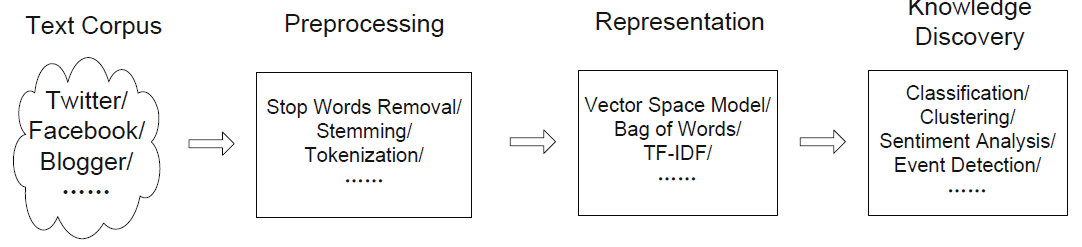
\includegraphics[height=0.25\linewidth, width=0.95\textwidth]{bilder/Abb2.png}
		\caption{Pipeline der Textklassifikation \citep{Kow19}  }\label{pipetk}
	\end{center}
\end{figure}
\subsection{Preprocessing}
Der rohe, unbehandelte Text wird beim \textit{Preprocessing} (deutsch: Vorbehandlung) in eine Form überführt, die eine nachfolgende Repräsentation der Daten durch Vektoren und ähnliche Methoden ermöglicht. Je nach gewünschter Anwendung sind hier verschiedene Vorverarbeitungsverfahren in Betracht zu ziehen.\\
Der Begriff Wortsegmentierung bzw. \textbf{Tokenisierung} bezeichnet die Zerteilung des Ausgangstexts in kleinere Einheiten, sogenannte \textit{Token} \citep{MannSch99}. In der Regel handelt es sich hierbei um einzelne Wörter, Zahlen und Satzzeichen. Als grundsätzliches Abgrenzungszeichen gelten in den meisten Sprachen die \textit{Whitespace}-Zeichen (Leerzeichen, Tab, Newline-Zeichen). Dies wird auch auf die zu analysierenden Tweets zutreffen, da diese fast ausschließlich in englischer Sprache verfasst sind.\\
\begin{figure}[htb]
	\begin{center}
		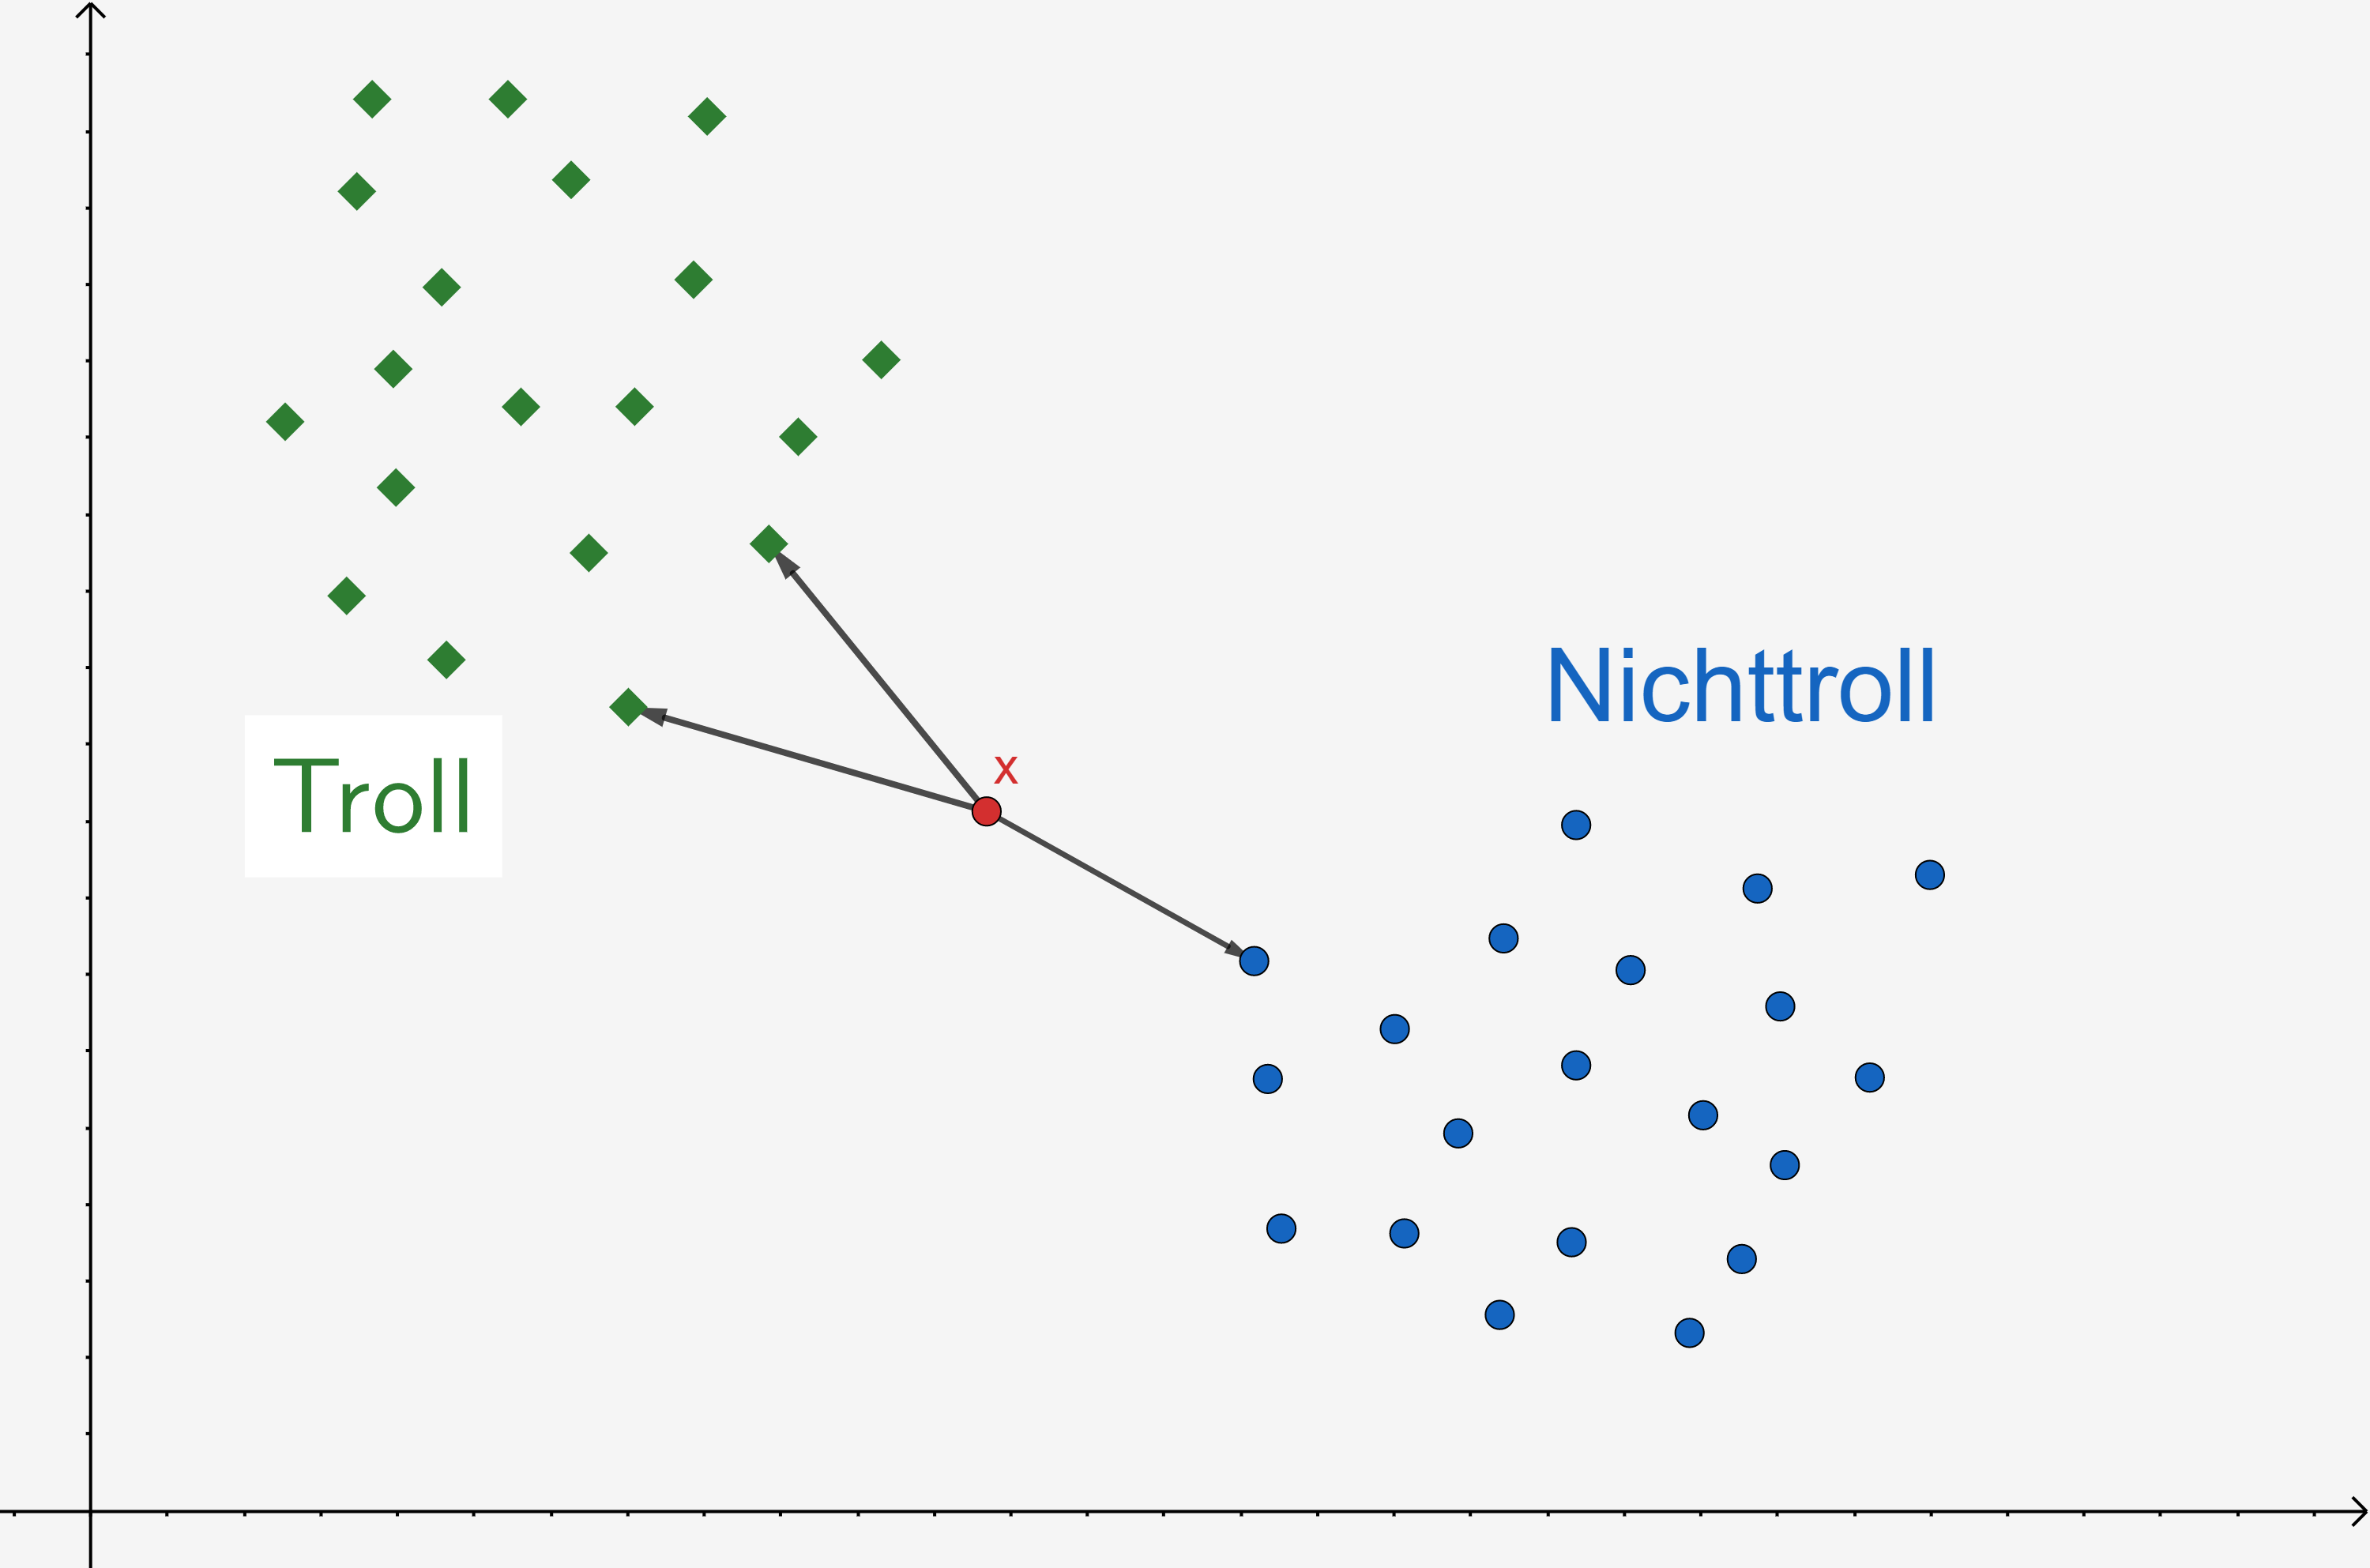
\includegraphics[width=\textwidth]{bilder/Abb3.png}
		\caption{Tokenisierung eines Beispielsatzes}\label{tokenization}
	\end{center}
\end{figure}\\
Eine weitere Methode der Vorverarbeitung ist das Entfernen von \textbf{Stoppwörtern}. Dies sind sehr häufig auftretende Wörter wie \glqq der\grqq, \glqq die\grqq, \glqq das\grqq, \glqq und\grqq{} oder \glqq von\grqq, welche vornehmlich eine grammatikalische Funktion und keinen Informationsgehalt haben. (vgl. ebd., S. 533)\\
Bei der \textbf{Lemmatisierung} \citep{Air06} werden mehrere Wörter unterschiedlicher Erscheinungsform, welche aber die gleiche Bedeutung haben, auf eine gemeinsame Grundform (genannt Lemma) zurückgeführt.  So lassen sich beispielsweise die deklinierten Substantive \glqq Wortes\grqq, \glqq Wörter\grqq, \glqq Wörtern\grqq auf \glqq Wort\grqq{} zurückführen, während die Grundform der konjugierten Verben \glqq schrieb\grqq, \glqq schreibe\grqq, \glqq schreibst\grqq{} und \glqq schreibt\grqq{} der Infinitiv \glqq schreiben\grqq ist. Ein verwandtes Konzept wird \textbf{Stemming} \citep{Air06} genannt. Der Unterschied zur Lemmatisierung besteht darin, dass das daraus resultierende Grundwort (hier: Stamm) kein natürlichsprachliches Wort sein muss, sondern in der Regel ein um Präfix und Suffix beschnittes Wort ist. Ein Beispiel hierfür ist die Reduzierung der Wörter \glqq gehen\grqq, \glqq umgehen\grqq und \glqq zugehen\grqq{} auf den Stamm \glqq geh-\grqq.\\
Für die Lemmatisierung eines Textes wird auch das \textbf{Part-of-Speech (POS) Tagging} \citep{Kuma15} benötigt. Hierbei wird einem Token seine Wortart (z.B. Nomen, Verb, Adjektiv) oder ein anderes Label wie \glqq Interpunktion\grqq{} zugewiesen. Werkzeuge, die dieses Verfahren anwenden, werden POS-\textit{Tagger} genannt.
\subsection{Feature Extraction}
Bevor eine Klassifikation vorgenommen werden kann, müssen die Merkmale aus den vorliegenden Texten gewonnen und mit mathematischen Methoden strukturiert bzw. modelliert werden. Hierbei fällt die Wahl zumeist auf Vektorisierung.\\
Die einfachste Vektorisierungstechnik ist die \textbf{Bag-of-Words} (BoW) \citep{Ramos13}. Hier wird ein Text durch einen Vektor mit den Begriffshäufigkeiten (auch: \textit{Term Frequencies} (\textbf{TF})) aller zuvor extrahierten Tokens des Textkorpus repräsentiert. Bei einem Beispielkorpus mit den beiden Texten \glqq my coffee is too hot\grqq{} und \glqq my tea is too cold\grqq{} und dem zuvor extrahierten Vokabular
\begin{flushleft}
	\hfil\{ "my", "coffee", "hot", "tea", "cold" \}
\end{flushleft}
ergibt sich die folgende Repräsentation:
\begin{flushleft}
	\hfil$v_1$ = [ 1, 1, 1, 0, 0 ]\\
	\hfil$v_2$ = [ 1, 0, 0, 1, 1 ]
\end{flushleft}
Eine Erweiterung dieser TF-Methode ist \textit{Term Frequency-Inverse Document Frequency} (\textbf{TF-IDF}) \citep{Ramos13}.  Hier wird die Vorkommenshäufigkeit anders gewichtet, um dem Aspekt gerecht zu werden, dass einige Begriffe überproportional oft vorkommen. Gleichung \ref{tfidf_weight} zeigt die Gewichtung 
\begin{equation}
	w(d,t) = TF(d,t) \cdot \log \left( \frac{N}{{DF}(t)} \right)
	\label{tfidf_weight}
\end{equation} 
wobei $N$ die Anzahl der Texte im Korpus und ${DF}(t)$ die Anzahl der Texte, welche den Begriff $t$ enthalten, ist.\\
Eine Möglichkeit, Wortkombinationen bzw. bestimmte Formulierungen als Merkmal zu berücksichtigen ist das \textbf{N-Gramm} \citep{Kow19}. Dies ist die Zusammenfassung von $N$ aufeinanderfolgenden Token in einem Text. Folglich handelt es sich bei den Elementen einer Bag of Words um 1-Gramme. Das nachfolgende Beispiel zeigt die Repräsentation des Textes \glqq Hier sehen Sie ein Beispiel.\grqq{} mit 2-Grammen:
\begin{flushleft}
	\hfil \{ \grqq Hier sehen \grqq, \grqq sehen Sie\grqq, \grqq Sie ein\grqq, \grqq ein Beispiel\grqq \}
\end{flushleft}
Alle vorausgegangenen Methoden der Merkmalsextraktion haben gemeinsam, dass sie keinen Aufschluss über Zusammenhänge der Wortbedeutungen (Semantik) geben. Dieses Problem versuchen die Techniken der \textbf{Worteinbettung} zu lösen. Ein prominentes Beispiel ist \textbf{Word2Vec} \citep{Mikolov13}. Die Grundidee ist hier, dass Begriffe, die eine ähnliche Bedeutung haben, in einem ähnlichen Kontext verwendet werden. Auf dieser Basis wird ein Vektor für jedes Wort im Vokabular durch ein neuronales Netz erzeugt. Die Entfernungen im daraus entstehenden Vektorraum geben dabei semantische Ähnlichkeiten wieder.
\subsection{Dimensionalitätsreduktion}
Bei sehr umfangreichen Datensätzen wie den mehr als 600.000 Tweets in dieser Arbeit werden in der Anwendung der zuvor beschriebenen Verfahren meist hochdimensionale Vektoren erzeugt. In der Folge werden viele Operationen bei späteren Algorithmen der Textklassifikation eine hohe Zeit- und Speicherkomplexität besitzen. Diesem Effekt versucht man im Voraus durch Dimensionalitätsreduktion entgegenzuwirken.\\
Ein erstes verwendetes Verfahren ist die Hauptkomponentenanalyse bzw. \textbf{Principal Component Analysis} (PCA) \citep{Jol02}. Mit diesem ist es möglich, in der Punktwolke der vorhandenen Vektoren all jene Vektor-Komponenten herauszufinden, die für die größte Varianz verantwortlich sind, also den größten Informationsgehalt haben. Der mathematische Mechanismus dahinter ist die Hauptachsentransformation: Es wird eine Ladungsmatrix aus den Eigenvektoren der Kovarianzmatrix gebildet, aus welcher der Anteil der Varianz jeder Komponente an der Gesamtvarianz ersichtlich ist. In der Folge können Komponenten, welche wenig Varianz beitragen, ohne nennenswerten Informationsverlust verworfen werden.\\
Eine andere Möglichkeit ist die \textbf{Nichtnegative Matrixfaktorisierung} (NMF) \citep{LeeSeung99}. Hier wird aus den $n$ Texten mit insgesamt $m$ Wörtern eine $m \times n$ Matrix gebildet, welche approximativ so faktorisiert wird, dass
\begin{center}
	$V \approx W H$
\end{center}
gilt, wobei W eine $m \times r$ Matrix und H eine $r \times n$ Matrix ist. Die $r$ Spalten von $W$ enthalten semantisch verwandte Wörter, welche zusammen einen Kontext bzw. ein Thema bilden. Voraussetzung für dieses Verfahren ist die Nichtnegativität von $V$.\pagebreak
\section{Klassifikationsverfahren}\label{clf}\raggedbottom
Nachdem die Tweets vorbearbeitet, die Merkmale gewonnen und die Dimensionen zwecks verbesserter Performance reduziert wurden, können sie nun als Trainingsdatensatz für ein Klassifikationsverfahren verwendet werden. Im nachfolgenden Kapitel werden verschiedene solcher Verfahren vorgestellt und im Hinblick auf Voraussetzungen, Stärken und Schwächen analysiert. Ein besonderes Augenmerk soll in der Analyse auf jenen Parametern liegen, welche die Ergebnisse beim vorliegenden Datensatz maßgeblich beeinflussen können.    
\subsection{k-Nearest-Neighbor-Algorithmus}
Der k-Nearest-Neighbor-Algorithmus (kNN) ist die erste hier behandelte Methode der Klassifikation \citep{Guo04}. Der zu klassifizierende Text wird zunächst analog zu den Trainingstexten vektorisiert. Über ein geeignetes Abstandsmaß werden nun die $k$ räumlich nächsten Nachbarn bestimmt. Der Text wird nun der Klasse zugeordnet, der die Mehrheit der Nachbarn angehören. Abbildung \ref{knn-alg} zeigt die k-Nearest-Neighbor-Klassifikation eines Punktes $x$ für $k=3$. Da die meisten Nachbarn hier dem Troll-Datensatz angehören, würde der zu $x$ gehörige Tweet somit als Troll-Tweet klassifiziert werden.\\
Die Wahl von $k$ ist entscheidend für die Qualität des Ergebnisses. Entscheidet man sich beispielsweise für ein zu kleines $k$, so ist möglich, dass vereinzelte Ausreißer die Genauigkeit trüben. Ist es auf der anderen Seite zu groß, so werden wahrscheinlich zu weit entfernte Punkte bei der Klassifikation miteinbezogen, was das Ergebnis wiederum verfälschen kann. Ferner ist bei Vorhandensein von 2 Klassen ein ungerades $k$ zu wählen, da andernfalls ein Unentschieden möglich ist.\\
\begin{figure}[htb]
	\begin{center}
		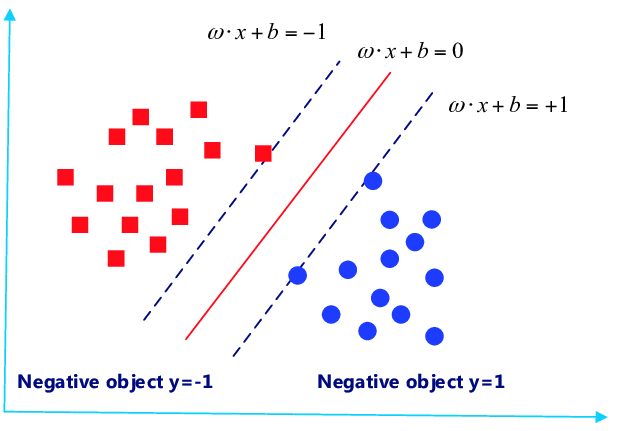
\includegraphics[scale=1.75]{bilder/Abb4.png}
		\caption{KNN-Klassifizierung für $k=3$}\label{knn-alg}
	\end{center}
\end{figure}\\
Eine zwingende Voraussetzung, um zuverlässig mit dem KNN-Algorithmus in diesem Projekt arbeiten zu können, ist die Dimensionalitätsreduktion. Die Merkmalsextraktion bringt bei den mehr als 600.000 Tweets hochdimensionale Vektoren hervor. Unbehandelt wären aufgrund der komponentenweisen Abstandsmessung Laufzeiten von einigen Minuten zu erwarten.\\
Die Vorteile dieses Verfahrens sind die einfache Implementierung und seine Eignung für alle möglichen Ausprägungen von Merkmalsräumen. Als Schwächen werden die bereits angesprochenen Probleme mit der Performance angesehen.
\subsection{Naiver Bayes-Klassifikator}
Der Naive Bayes-Klassifikator (NB) ist ein statistisches Verfahren der Klassifikation \citep{Rish01}. Die Grundlage der Berechnung bildet hier der Satz von Bayes, bekannt aus der Wahrscheinlichkeitstheorie. In seiner herkömmlichen Interpretation beschreibt dieser die Berechnung der Wahrscheinlichkeit, dass ein Ereignis dem anderen vorausgegangen ist. Wendet man dies auf einen gegebenen Text $t \in T$ und die Klasse $k_i \in K$ an, so erhält man die Formel für die Wahrscheinlichkeit, dass $t$ der Klasse $k_i$ angehört (siehe Gleichung \ref{bayes}).
\begin{equation}
	P(k_i|t) = \frac{P(t|k_i) \cdot P(k_i)}{P(t)}
	\label{bayes}
\end{equation}
Der Klassifikator bestimmt nun diejenige Klasse $k_i$, für die der Wert dieser Formel maximal ist. Mathematisch formuliert:
\begin{equation}
	k = arg \max\limits_{k_i \in K} P(k_i|t) = arg \max\limits_{k_i \in K} \frac{P(t|k_i) \cdot P(k_i)}{P(t)}
\end{equation}
Die Werte für $P(k_i)$ und $P(t)$ werden a priori über relative Anteilshäufigkeiten, also über den Anteil einer Klasse und den Anteil eines Textes am gesamten Merkmalraum, bestimmt. Für die Maximierung wird meist die Maximum-Likelihood-Methode benutzt.\\
Jeder Klasse wird vor der Klassifizierung eine bestimmte Form der Wahrscheinlichkeitsverteilung, meist eine Normalverteilung, und die stochastische Unabhängigkeit der Merkmale unterstellt. Letztere Annahme ist \glqq naiv\grqq{}  weil nicht immer zutreffend, der Algorithmus liefert in der Praxis bei vielen Anwendungen dennoch solide Ergebnisse. Wird diese Annahme hingegen durch stark korrelierte Daten gröber verletzt, so sind Genauigkeitsverluste zu erwarten, was eine Schwäche dieses Verfahrens ist. Im Rahmen der Evaluation werden Ergebnisse unter Annahme einer Normalverteilung, einer Multinomialverteilung und einer komplementären Verteilung nach \citet{rennie03} verglichen.
\pagebreak
\subsection{Support Vector Machine}\label{svm}
Ein anderes Lernmodell trägt den Namen Support Vector Machine (SVM) \citep{Nayak15}. Die Grundidee ist hier, die vorliegenden Klassen im multidimensionalen Raum durch Einschub einer Hyperebene räumlich zu trennen. Die Ebene wird dabei so platziert, dass der Abstand zu den nächstliegenden Vektoren der beiden Klassen, den sogenannten Stützvektoren (engl. \textit{support vectors}) maximal ist. Abbildung \ref{svm-alg} zeigt beispielhaft zwei solcher durch eine Hyperebene (rote Gerade) getrennte Klassen in einem zweidimensionalen Merkmalraum. 
\begin{figure}[htb]
	\begin{center}
		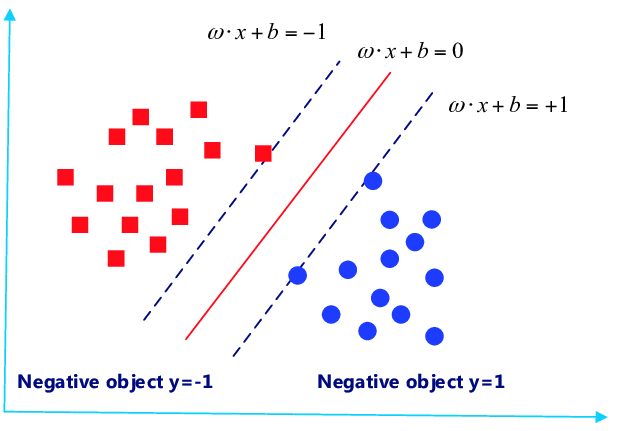
\includegraphics[scale=0.75]{bilder/Abb5.png}
		\caption{SVM-Klassifizierung \citep{Zhou16}}\label{svm-alg}
	\end{center}
\end{figure}\\
 Für ein zu klassifizierendes Objekt wird nun mithilfe einer Entscheidungsfunktion festgestellt, auf welcher Seite der Ebene es liegt und kann so eindeutig einer Klasse zugeordnet werden. Ist der Einschub einer Hyperebene nicht möglich, d.h. sind die Klassen nicht linear trennbar, so behilft man sich mit dem sogenannten \glqq Kernel-Trick\grqq{}: Der Merkmalraum wird auf einen höherdimensionalen Raum abgebildet, in welchem die Klassen dann linear trennbar sind. Diese Transformation benötigt eine hohe Rechenleistung und stellt deshalb bei stark überlappenden Klassen eine Schwäche dieses Verfahrens dar. Bei weniger überlappenden oder linear trennbaren Klassen ist der Algorithmus in der Einstufung jedoch sehr schnell. Ein weiterer Vorteil ist der relativ geringe Speicherverbrauch, da zur Klassifikation nur ein Teil der Trainingsdaten gebraucht wird.\\
 Ein Parameter, der die Ergebnisse beeinflussen kann, ist der Bestrafungsparameter $C$. Dieser gibt an, wie stark die Gefahr der Falschklassifizierung berücksichtigt werden soll. Je niedriger der Wert, desto leichter wird es, eine Trennung zu vollziehen und dabei einzelne Ausreißer zu ignorieren. Allerdings findet dann bei mäßiger bis starker Überlappung keine eindeutige Trennung der Klassen statt. Je höher der Wert, desto strenger versucht der Algorithmus, alle Punkte in der Entscheidung miteinzubeziehen. Hier besteht die Gefahr der Überanpassung.
\subsection{Entscheidungsbäume}\label{tree}
Die Grundlage für ein weiteres Klassifikationsverfahren sind die sogenannten Entscheidungsbäume (engl. \textit{decision trees}) \citep{rokach05}. Hierbei handelt es sich um herkömmliche, aus der Graphentheorie bekannte Bäume, welche eine Entscheidungsfolge abbilden. Für jedes zu klassifizierende Objekt wird der Baum einmal durchlaufen. An jedem inneren Knoten wird nun der Wert eines extrahierten Merkmals abgefragt. Je nach Ergebnis des Vergleichs wird entschieden, welches Kind als nächstes besucht wird. Die Blätter beinhalten die möglichen Klassen, sodass nach der letzten Entscheidung mit Ankommen am Ende des Baumes die Klassifikation vollzogen ist. Abbildung \ref{dtree} zeigt beispielhaft einen Entscheidungsbaum für die Klassifikation eines Messestandorts anhand von drei Merkmalen. Die möglichen Klassen für einen Standort sind \glqq geeignet\grqq{} und \glqq ungeeignet\grqq{}.
\begin{figure}[htb]
	\begin{center}
		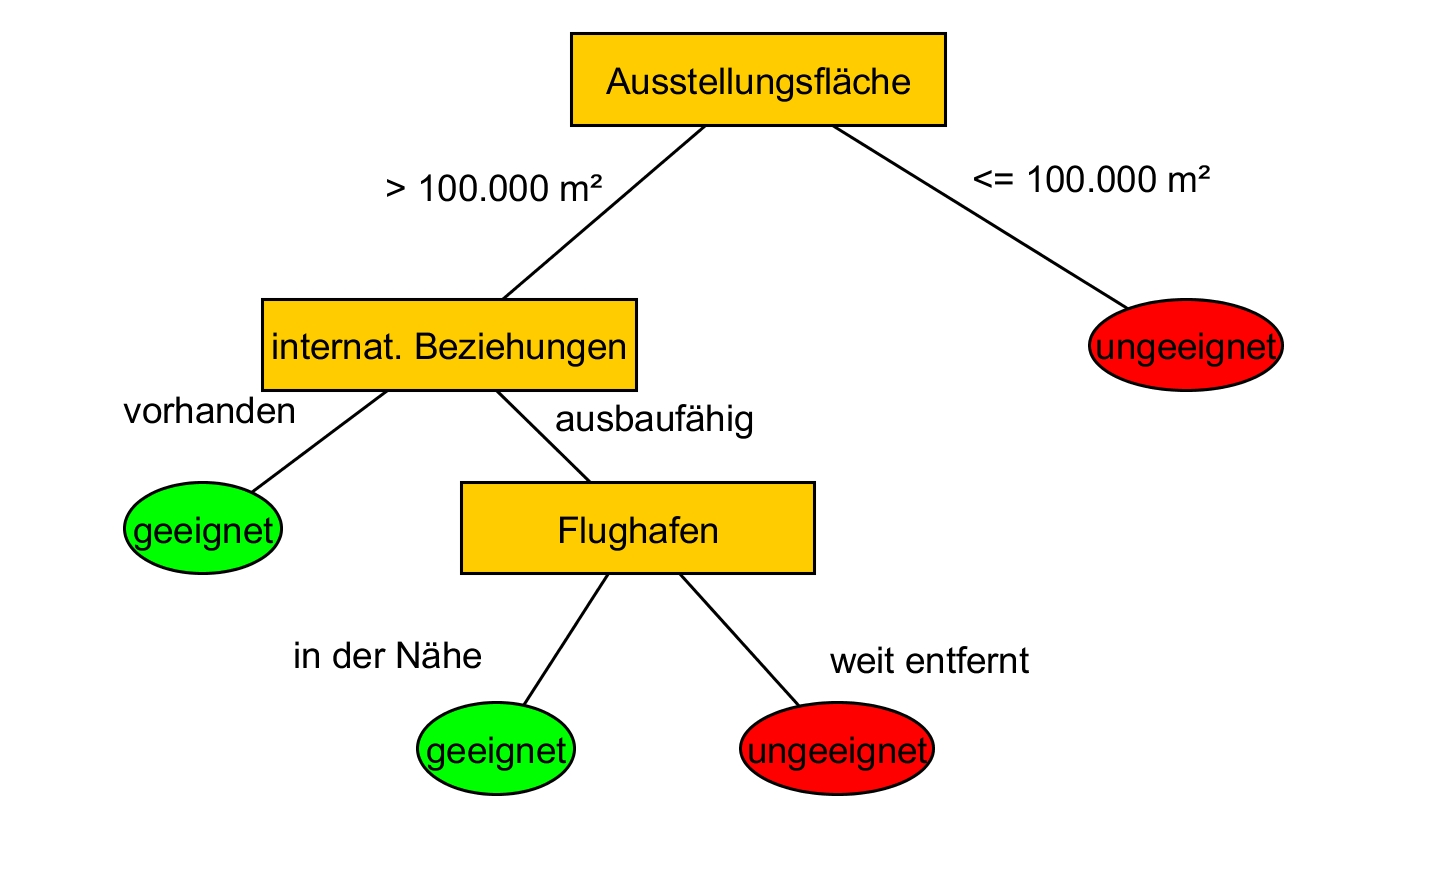
\includegraphics[scale=0.25]{bilder/Abb6.jpg}
		\caption{Entscheidungsbaum zur Klassifizierung eines Messestandorts}\label{dtree}
	\end{center}
\end{figure}\\
Das Training bzw. das Lernen besteht bei diesem Verfahren im Aufbau des Baumes. Beginnend bei der Wurzel wird nun dasjenige Merkmal bestimmt, welches den größten Fortschritt in der Klassifikationsentscheidung bringt. Ein gebräuchliches Maß dafür ist die \textit{Gini Impurity}, welche die Homogenität bzw. Heterogenität der Daten anzeigt. Gleichsam anwendbar ist hier auch die Entropie, welche den mittleren Informationsgehalt des Merkmalvektors misst. Das gefundene Merkmal dient nun zur Aufteilung der ursprünglichen Datenmenge. Auf die neu entstehenden Mengen wird diese Methode nun rekursiv angewendet bis Mengen erzeugt werden, deren Elemente alle der gleichen Klasse angehören.\\
Durch die klare Strukturierung und grafische Darstellbarkeit ist die Entscheidungsbaum-Klassifikation als Konzept leicht verständlich. Ein weiterer Vorteil ist eine automatische Merkmalfilterung beim Aufbau des Baums: Merkmale, die durch Gini Impurity bzw. Entropie als irrelevant erkannt wurden, können leicht weggelassen werden. Hier sind Zeit- und Speichergewinne möglich.\\
Eine Schwäche dieses Verfahrens ist die schwache Robustheit der Entscheidungsbäume. Dies bedeutet, dass kleine Änderungen im Ausgangsdatensatz zu sehr großen Veränderungen in der Datenstruktur und der anschließenden Klassifikation führen können.
\subsection{Mehrschichtiges Perzeptron}\label{mlp}
Das mehrschichtige Perzeptron (engl. \textit{multi-layer perceptron, MLP}) ist ein Vertreter der künstlichen neuronalen Netze \citep{du2014}. In seinem grundlegenden Aufbau ähnelt es einem Logikgatter. Die grundlegenden Bausteine, analog zu Gehirnzellen Neuronen genannt, sind in Schichten angeordnet. Die Eingabeschicht nimmt den Merkmalvektor komponentenweise entgegen, während die Neuronen der Ausgabeschicht das Klassifikationsergebnis ausgeben. Die dazwischenliegenden Schichten werden versteckte Schichten bzw. \textit{hidden layers} genannt. Abbildung \ref{mlp-ex} illustiert ein Beispiel für Netz, welches einen vierdimensionalen Vektor verarbeitet.\\
 \begin{figure}[htb]
	\begin{center}
		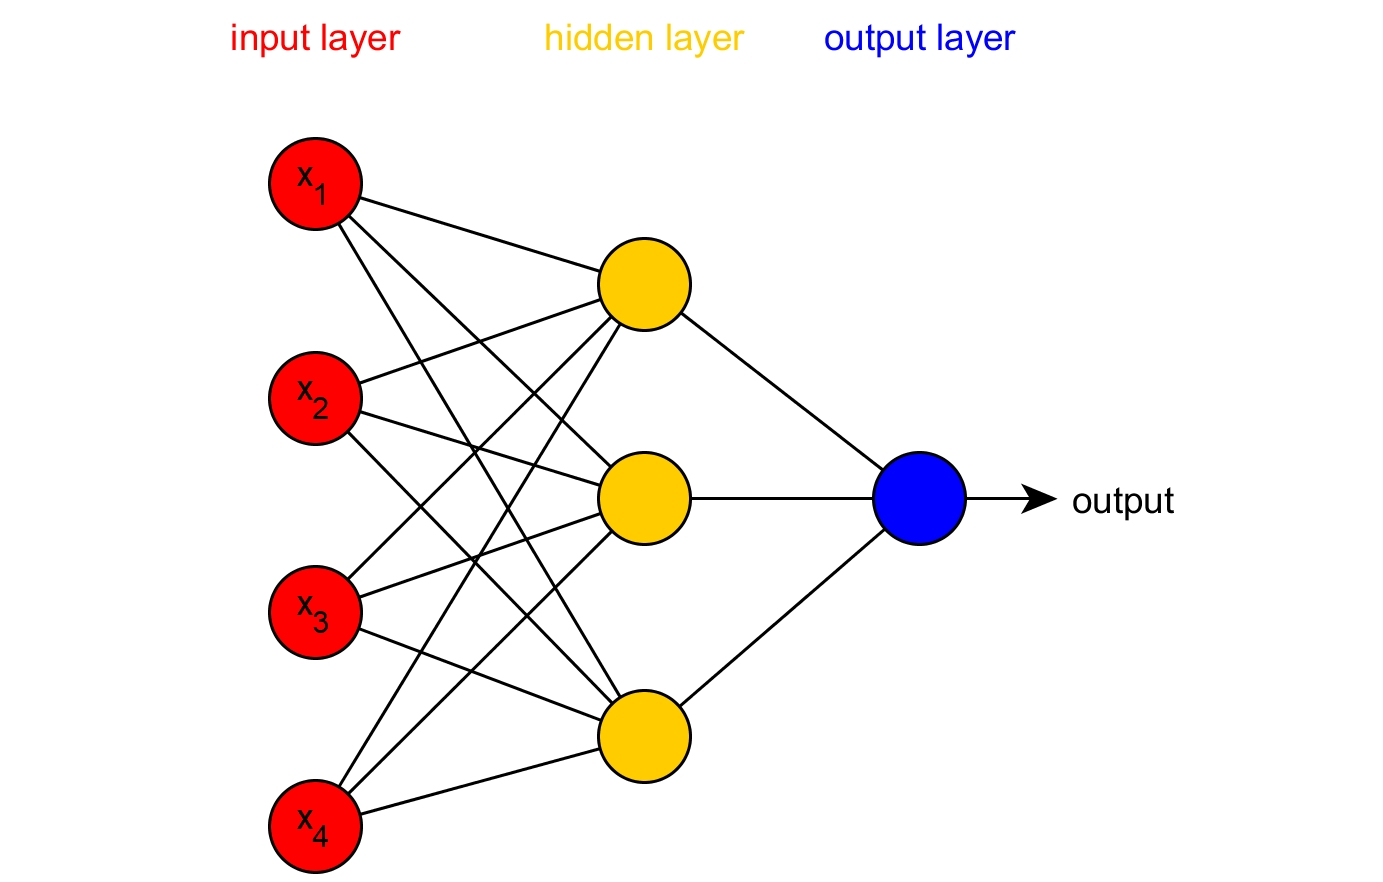
\includegraphics[scale=0.20]{bilder/Abb7.jpg}
		\caption{Beispiel für mehrschichtiges Perzeptron}\label{mlp-ex}
	\end{center}
\end{figure}\\
Jedes Neuron einer Schicht hat eine Verbindung, ähnlich einer Kante, zu einem Neuron (oft auch zu allen) der nächsten Schicht. Die Verbindung trägt ein Gewicht. Dazu trägt auch jedes Neuron einer versteckten Schicht und der Output-Schicht ein sogenanntes Verzerrungsgewicht bzw. \textit{bias weight} $b$.\\
 Der Lernprozess läuft nun wie folgt ab: Beginnend bei den Input-Neuronen wird für jede Eingabe eine gegebene Aktivierungsfunktion berechnet. Das Ergebnis wird an die nachfolgenden Neuronen weitergeschickt und erneut die Aktivierungsfunktion berechnet. Ist es schließlich in der Output-Schicht angekommen, so wird das Ergebnis interpretiert und mit der vorher deklarierten Klasse verglichen. Ist das Ergebnis falsch, so werden die Gewichte des Netzes von hinten nach vorne neujustiert. Man spricht hier von \textit{Backpropagation}. Auf diese Weise lernt das Netz mit jedem Fehler dazu und die Klassifikation wird zunehmend genauer.\\
 Als Aktivierungsfunktion werden klassischerweise drei verschiedene Funktionen herangezogen \citep{nwankpa2018activation}. Die erste Funktion ist der \textit{Tangens hyperbolicus} (kurz tanh).
 \begin{equation}
 	tanh(x) = \frac{sinh(x)}{cosh(x)} = \frac{e^x - e^{-x}}{e^x + e^{-x}}
 \end{equation}
 Oft verwendet wird auch die folgende logistische Funktion
 \begin{equation}
 	f(x) = \frac{1}{1 + e^{-x}}
 \end{equation}
 Eine neuere Form der Aktivierungsfunktion ist die \textit{rectified linear unit} (kurz: ReLu). Sie ist folgendermaßen definiert:
 \begin{equation}
 	f(x) = \max(0, x)
 \end{equation}
\pagebreak
\section{Evaluation}\raggedbottom
Im nachfolgenden Kapitel sollen nun die Ergebnisse der praktischen Anwendung der Klassifikationstechniken auf die vorliegenden Datensätze ausgewertet werden. Wie in den vorangegangenen Kapiteln besprochen, wird erwartet, dass verschiedene Techniken der Merkmalsextraktion, verschiedene Level der Dimensionalitätsreduktion und verschiedene Hyperparametereinstellungen die Ergebnisse qualitativ beeinflussen werden. Eine Methode, die es ermöglicht, diese Unterschiede zu messen und gleichzeitig die beste Kombination zu bestimmen, ist die sogenannte Hyperparameteroptimierung. Hierbei ...

\subsection{Implementierung} 
Zwecks Nachvollziehbarkeit und Transparenz soll an dieser Stelle kurz auf die parallel erfolgte praktische Anwendung der beschriebenen Techniken eingegangen werden.\\
Im Rahmen dieser Abschlussarbeit wurde ein Kommandozeilen-Tool namens \glqq TrollDetector\grqq{} \footnote{\url{https://github.com/rokoe102/trolldetector}} in der Programmiersprache Python entwickelt. Dieses hat mehrere Funktionen. Zum einen ist damit möglich, ein beliebiges Klassifikationsverfahren mit selbst gewählten Hyperparametern auf den Datensatz anzuwenden. Dies geschieht nach dem bereits erwähnten \glqq Train-and-Test\grqq-Verfahren. Hier sind auch Merkmalsextraktion (z.B. TF vs. TF-IDF) und Dimensionalitätsreduktion direkt steuerbar.\\
Eine weitere Funktion ist die Hyperparameteroptimierung für jedes Verfahren mit anschließender Auswertung der Ergebnisse. Für die Optimierung wird eine Rastersuche verwendet. Bei dieser Methode wird das jeweilige Klassifikationsverfahren auf einer fest definierten Untermenge aller möglichen Kombinationen von Hyperparametern ausgeführt. Anschließend werden die Ergebnisse der Kombinationen ausgewertet.\\
Schließlich ist es mit dem Programm noch möglich, einen Vergleich der fünf Klassifikatoren anzustellen. Die voreingestellten Hyperparameter sind jene, welche bei der Hyperparameteroptimierung am besten abgeschnitten haben, sodass eine Vergleichbarkeit hergestellt wird.\\
Zur Verarbeitung und Klassifikation des Datensatzes wurden ausschließlich Klassen und Funktionen aus der \glqq scikit-learn\grqq-Bibliothek von \citet{scikit-learn} verwendet.
\pagebreak\pagebreak
\subsection{Hyperparameteroptimierungen}
Zu Beginn soll jedes Verfahren einzeln auf die Eignung als Trollerkennungsinstrument untersucht werden. Hierzu werden die Ergebnisse der Hyperparameteroptimierungen diskutiert. Folgende Hyperparameter teilen sich dabei alle Verfahren, da die Merkmalsextraktion bei ihnen gleich abläuft:
\begin{table}[htb]
	\begin{center}
		\begin{tabular}{|c|c|}
			\hline
			Hyperparameter & gewählte Werte \\ \hline \hline
			Merkmalgewichtung & TF, TF-IDF \\ \hline
			Stoppwort-Filterung & keine, englisch\\ \hline
			n-Gramm-Extraktion & 1-Gramme, 1+2-Gramme\\ \hline			
		\end{tabular}
		\caption{gemeinsame Hyperparameter aller Verfahren}\label{common-params}
	\end{center}
\end{table}\\
Alle anderen Parameter sind verfahrensspezifisch.
\subsubsection{k-Nearest-Neighbor-Algorithmus}
Beim KNN-Algorithmus sind neben den Hyperparametern, welche mit anderen Verfahren geteilt werden, die Abstandsmetrik und der k-Wert für die zu untersuchenden Nachbarn gegeben.\\
Tabelle \ref{results-knn} zeigt die mittleren Ergebnisse verschiedener Ausprägungen aller Hyperparameter einerseits im Vergleich untereinander und im Vergleich zur durchschnittlichen und zur besten Performance. Hieraus lassen sich verschiedene Schlussfolgerungen ziehen:\\
\begin{table}[htb]
	\begin{center}
		\begin{tabular}{|c|c|c|c|c|c|c|}
			\hline 
			Hyperparameter & Genauigkeit & Relevanz & Segreganz & Sensitivität & Spezifität & $F_1$ \\ \hline \hline
			TF & \textbf{0.951} & \textbf{0.937} & 0.965 & 0.964 & \textbf{0.937} & \textbf{0.949} \\ \hline
			TF-IDF  & 0.949 & 0.932 & \textbf{0.966} & 0.964 & 0.935 & 0.948 \\ \hline \hline
			engl. Stoppwörter  & 0.947 & 0.931 & 0.962 & 0.961 & 0.934 & 0.946 \\ \hline
			keine Filterung  & \textbf{0.953} & \textbf{0.937} & \textbf{0.968} & \textbf{0.967} & \textbf{0.940} & \textbf{0.952} \\ \hline \hline
			1-Gramme  & \textbf{0.955} & \textbf{0.941} & \textbf{0.969} & \textbf{0.967} & \textbf{0.967} & \textbf{0.954} \\ \hline 
			1+2-Gramme  & 0.945 & 0.928 & 0.962 & 0.961 & 0.961 & 0.944 \\ \hline \hline
			$k = 5$  & \textbf{0.953} & \textbf{0.938} & \textbf{0.967} & \textbf{0.966} & \textbf{0.940} & \textbf{0.952} \\ \hline 
			$k = 15$  & 0.950  & 0.934  & 0.965  & 0.964 & 0.936  & 0.949 \\ \hline 
			$k = 25$  & 0.948  & 0.931  & 0.964  & 0.962 & 0.934  & 0.947  \\ \hline \hline
			euklid. Metr.  & 0.950 & \textbf{0.935} & 0.965 & 0.963 & 0.937 & 0.949 \\ \hline
			Manhattan  & 0.950 & 0.934 & \textbf{0.966} &\textbf{0.964} & 0.937 & 0.949 \\ \hline
			 \hline
			Maximum  & 0.960 & 0.948 & 0.973 & 0.972 & 0.950 & 0.959 \\ \hline
			durchschnittl. & 0.950 & 0.934 & 0.965 & 0.964 & 0.937 & 0.949 \\ \hline
		\end{tabular}
		\caption{Ergebnisse bei KNN}\label{results-knn}
	\end{center}
\end{table}\\\\
Insgesamt sind beim KNN-Algorithmus ausgezeichnete Zahlen zu beobachten. Im Maximum liegen  nahezu alle Kennzahlen über 95\%, positiv auffallend sind hier Werte der Segreganz und der Sensitivität von über 97\%. Durchschnittlich werden immer Punktzahlen von über 93\% erreicht. Ein Unterschied im Abschneiden unterschiedlicher Parametereinstellungen ist bei der Merkmalsgewichtung zu erkennen: TF erreicht hier ein wenig bessere Punktzahlen als TF-IDF. Die Filterung von englischen Stoppwörtern bringt im Mittel keine Verbesserung hervor. Extrahiert man nur 1-Gramme, anstatt 1-Gramme und 2-Gramme, erreicht man bis zu 1\% höhere Punktzahlen.\\
Bei den verfahrensspezifischen Hyperparametern gibt es nur wenige Schwankungen. Beim k-Wert deutet sich an, dass ein einstelliger Wert besser abschneidet als ein zweistelliger, die Verbesserungen belaufen sich aber nur auf höchstens 0,5\%. Bei den Metriken ist auffällig, dass unterschiedliche Arten der Abstandsmessungen nahezu keinen Unterschied in der Qualität hervorbringen, die Abweichungen betragen hier höchstens 0,1\%.\\
Angesichts seiner durchweg hohen Punktzahlen in allen möglichen Gütemaßen ist der k-Nearest-Neighbor-Algorithmus sehr gut für die Erkennung von IRA-ähnlichen Trollen geeignet.
\subsubsection{Naiver Bayes-Klassifikator}
Der einzige verfahrensspezifische Hyperparameter des Naiven Bayes-Klassifikators ist die angenommene Verteilung der Merkmalvektoren. Getestet wurde mit einer Normalverteilung, einer Multinomialverteilung und einer komplementären Verteilung nach >Rennie et al. (2003)<.\\
Die Ergebnisse in Tabelle \ref{results-nb} lassen folgende Schlüsse zu:\\
Dieses Verfahren schneidet je nach Parameter-Einstellung sehr unterschiedlich ab. So liefert die Annahme einer Normalverteilung oder einer komplementären Verteilung Punktzahlen von 75 - 85\%.
\begin{table}[htb]
	\begin{center}
		\begin{tabular}{|c|c|c|c|c|c|c|}
			\hline 
			Hyperparameter & Genauigkeit & Relevanz & Segreganz & Sensitivität & Spezifität & $F_1$ \\ \hline \hline
			TF         & \textbf{0.747} & 0.772 & \textbf{0.767} & \textbf{0.685} & 0.804 & \textbf{0.694} \\ \hline
			TF-IDF     & 0.702 & \textbf{0.798} & 0.736 & 0.571 & \textbf{0.824} & 0.536 \\ \hline \hline
			engl. Stoppwörter  & 0.715 & 0.751 & 0.731 & 0.620 & 0.803 & \textbf{0.616} \\ \hline
			keine Filterung    & \textbf{0.734} & \textbf{0.819} & \textbf{0.77}1 & \textbf{0.636} & \textbf{0.825} & 0.614 \\ \hline \hline
			1-Gramme    & 0.735 & 0.811 & 0.761 & 0.642 & 0.642 & 0.631 \\ \hline 
			1+2-Gramme  & 0.713 & 0.758 & 0.741 & 0.613 & 0.613 & 0.599 \\ \hline \hline
			Normal      & 0.807 & 0.762 & 0.868 & 0.878 & 0.741 & 0.815 \\ \hline 
			Multinomial & 0.585 & 0.841 & 0.568 & 0.198 & 0.947 & 0.253 \\ \hline 
			Komplementär& 0.781 & 0.752 & 0.818 & 0.808 & 0.755 & 0.777  \\ \hline 
			\hline
			Maximum        & 0.834 & 1.000 & 0.949 & 0.958 & 1.000 & 0.855 \\ \hline
			durchschnittl. & 0.724 & 0.785 & 0.751 & 0.628 & 0.814 & 0.615 \\ \hline
		\end{tabular}
		\caption{Ergebnisse bei NB}\label{results-nb}
	\end{center}
\end{table}\\
Bei einer Multinomialverteilung sind die Ergebnisse im Durchschnitt deutlich schlechter. Beispielsweise ist die mittlere Treffergenauigkeit 58,5\% und die mittlere Sensitivität bei nur 19,8\%. Es gibt hierbei sehr starke, gleichzeitige Ausreißer nach oben und unten: In Kombination mit TF-IDF wird eine Spezifität von 100\% bei einer Sensitivität von 0\% erreicht, weshalb die Treffergenauigkeit hier etwa 50\% beträgt.\\
Bei der Merkmalgewichtung schneiden TF und TF-IDF in einer Hälfte der Gütemaße besser ab. Das Unterlassung einer Filterung von englischen Stoppwörtern führt auch bei diesem Verfahren zu leicht besseren Ergebnissen von 2 - 6\%.\\
Lässt man die Annahme einer Multinomialverteilung außen vor, so werden mit dieser Methode Punktzahlen von durchschnittlich 75\% - 85\% erreicht, was gerade mit Einstellung der richtigen Hyperparameter zu relativ verlässlichen Ergebnissen führt. Unter diesen Voraussetzungen ist das Verfahren zur Trollerkennung durchaus geeignet.
\subsubsection{Support Vector Machine}
Die Klassifikation mit einer Support Vector Machine hat wie in Kapitel \ref{svm} beschrieben den Bestrafungsparameter C als einzigen verfahrensspezifischen Hyperparameter. Bei Ausführung der Optimierung kommen folgende Ergebnisse (Tabelle \ref{results-svm}) zustande:\\
Insgesamt liefert die SVM im Mittel Punktzahlen von mindestens 80\% in allen betrachteten Gütemaßen. Beste Werte sind Segreganz und Sensitivität: Durchschnittlich werden hier ca. 93\% und im Maximum 97\% erreicht.\\
Unterschiedliche Merkmalgewichtungen führen auch hier zu unterschiedlichen Ergebnissen. Sowohl TF als auch TF-IDF schneiden in drei von sechs Gütemaßen besser ab als das jeweils andere. Der stärkste Unterschied betrifft Segreganz und Sensitivität: Hier schneidet TF 6\% besser ab. Bei allen anderen Arten der Merkmalsextraktion gibt es nur wenige Schwankungen von höchstens 2\%.\\
Beim Bestrafungsparameter C sind bis auf 0,1\% keine Schwankungen in den unterschiedlichen Ausprägungen auszumachen.\\
\begin{table}[htb]
	\begin{center}
		\begin{tabular}{|c|c|c|c|c|c|c|}
			\hline 
			Hyperparameter & Genauigkeit & Relevanz & Segreganz & Sensitivität & Spezifität & $F_1$ \\ \hline \hline
			TF         & \textbf{0.875} & 0.813 & \textbf{0.959} & \textbf{0.964} & 0.793 & 0.882 \\ \hline
			TF-IDF     & 0.868 & \textbf{0.838} & 0.900 & 0.900 & \textbf{0.837} & \textbf{0.868} \\ \hline \hline
			engl. Stoppwörter  & 0.865 & 0.816 & 0.929 & 0.931 & 0.804 & 0.869 \\ \hline
			keine Filterung    & \textbf{0.878} & \textbf{0.834} & \textbf{0.930} & \textbf{0.933} & \textbf{0.826} & \textbf{0.880} \\ \hline \hline
			1-Gramme   & 0.870 & 0.820 & \textbf{0.932} & \textbf{0.935} & \textbf{0.935} & 0.874 \\ \hline
			1+2-Gramme  & \textbf{0.873} & \textbf{0.830} & 0.928 & 0.929 & 0.929 & \textbf{0.876} \\ \hline \hline
			$C=1.00$ & 0.872 & 0.826 & 0.930 & 0.932 & 0.815 & 0.875 \\ \hline 
			$C=0.75$ & 0.871 & 0.825 & 0.929 & 0.932 & 0.815 & 0.875 \\ \hline 
			$C=0.50$ & 0.871 & 0.825 & 0.930 & 0.932 & 0.814 & 0.875 \\ \hline
			\hline
			Maximum        & 0.892 & 0.867 & 0.970 & 0.974 & 0869 & 0.892 \\ \hline
			durchschnittl. & 0.871 & 0.825 & 0.930 & 0.932 & 0.815 & 0.875 \\ \hline
		\end{tabular}
		\caption{Ergebnisse bei SVM}\label{results-svm}
	\end{center}
\end{table}\\
Insgesamt ist die SVM-Klassifikation mit den erreichten Punktzahlen ziemlich verlässlich und daher für die Trollerkennung gut geeignet. Von Vorteil ist auch, dass die durchweg hohe Segreganz für ein niedriges $f_n$ spricht, was eine konservative Klassifikation, welche für die Trollerkennung wichtig ist, gewährleistet. Eine positive Eigenschaft ist außerdem die Stabilität des Verfahrens: Selbst mit wenigen bewussten oder zufälligen Einstellungen liefert das Verfahren immer noch gute Ergebnisse, was für eine Art Benutzerfreundlichkeit spricht.
\subsubsection{Entscheidungsbäume}
Bei der Entscheidungsbaum-Klassifikation sind neben den von allen geteilten Hyperparametern auch das Aufteilungskriterium gegeben. Die zwei Möglichkeiten sind hier die in Kapitel \ref{tree} beschriebenen Maße Gini Impurity und Entropie. Aus Tabelle \ref{results-tree} lassen sich folgende Schlüsse ziehen:\\
Die Klassifikation erreicht im Mittel in allen Gütekriterien sehr hohe Werte von 94\%. Die maximalen Werte liegen mit ca. 95\% nur 1\% darüber. Es lässt sich aus diesem Grund leicht erkennen, dass hier nur sehr geringe Schwankungen vorhanden sind. Dies ist auch im Vergleich unter den Hyperparametern zu erkennen: Zwischen TF und TF-IDF, der Filterung englischer Stoppwörter und keiner Filterung und der Auswahl der jeweiligen n-Gramme liegen jeweils nur 1\% Unterschied. Die Aufteilungskriterien Gini Impurity und Entropie unterscheiden sich nur um 0,2\%.\\
Diese ausgezeichneten Punktzahlen legen nahe, dass eine zuverlässige Trollerkennung mit diesem Verfahren sehr gut zu leisten ist. Sowohl die geringen Schwankungen unter den Hyperparametern, als auch die geringen Unterschiede in den Gütekriterien sprechen für eine hohe Stabilität des Verfahrens. Dies bedeutet auch hier, dass selbst zufällige Einstellungen niemals zu schlechten Ergebnissen führen können.\\
\begin{table}[htb]
	\begin{center}
		\begin{tabular}{|c|c|c|c|c|c|c|}
			\hline 
			Hyperparameter & Genauigkeit & Relevanz & Segreganz & Sensitivität & Spezifität & $F_1$ \\ \hline \hline
			TF       & 0.945 & 0.938 & 0.951 & 0.948 & 0.941 & 0.943 \\ \hline
			TF-IDF   & 0.936 & 0.930 & 0.941 & 0.937 & 0.934 & 0.934 \\ \hline \hline
			engl. Stoppwörter & 0.938 & 0.932 & 0.943 & 0.939 & 0.936 & 0.936 \\ \hline
			keine Filterung    & 0.942 & 0.935 & 0.949 & 0.946 & 0.939 & 0.941 \\ \hline \hline
			1-Gramme   & 0.944 & 0.937 & 0.951 & 0.948 & 0.948 & 0.943 \\ \hline
			1+2-Gramme  & 0.936 & 0.931 & 0.941 & 0.937 & 0.937 & 0.934 \\ \hline \hline
			Gini & 0.939 & 0.933 & 0.945 & 0.942 & 0.937 & 0.937 \\ \hline
			Entropie & 0.941 & 0.935 & 0.947 & 0.944 & 0.939 & 0.939 \\ \hline
			\hline
			Maximum        & 0.950 & 0.944 & 0.957 & 0.954 & 0.947 & 0.949 \\ \hline
			durchschnittl. & 0.940 & 0.934 & 0.946 & 0.943 & 0.938 & 0.938 \\ \hline
		\end{tabular}
		\caption{Ergebnisse der Entscheidungsbaum-Klassifikation}\label{results-tree}
	\end{center}
\end{table}\\
\subsubsection{Mehrschichtiges Perzeptron}
Der wichtigste einstellbare Hyperparameter bei der Klassifikation mit einem Mehrschichtigen Perzeptron ist die Aktivierungsfunktion. Bei der Hyperparameteroptimierung wurden die drei in Kapitel \ref{mlp} beschriebenen Aktivierungsfunktionen getestet.
\begin{table}[htb]
	\begin{center}
		\begin{tabular}{|c|c|c|c|c|c|c|}
			\hline 
			Hyperparameter & Genauigkeit & Relevanz & Segreganz & Sensitivität & Spezifität & $F_1$ \\ \hline \hline
			TF       & \textbf{0.904} & 0.868 & \textbf{0.947} & \textbf{0.948} & 0.863 & \textbf{0.906} \\ \hline
			TF-IDF   & 0.888 & 0.868 & 0.909 & 0.907 & \textbf{0.870} & 0.887 \\ \hline \hline
			engl. Stoppwörter & 0.891 & 0.862 & 0.925 & 0.924 & 0.860 & 0.892 \\ \hline 
			keine Filterung   & \textbf{0.901} & \textbf{0.873} & \textbf{0.931} & \textbf{0.931} & \textbf{0.873} & \textbf{0.901} \\ \hline\hline
			1-Gramme   & \textbf{0.898} & 0.868 & \textbf{0.932} & \textbf{0.932} & \textbf{0.932} & \textbf{0.898} \\ \hline
			1+2-Gramme  & 0.894 & 0.868 & 0.925 & 0.923 & 0.923 & 0.894 \\ \hline \hline
			relu & \textbf{0.931} & \textbf{0.917} & \textbf{0.945} & \textbf{0.942} & \textbf{0.920} & \textbf{0.929} \\ \hline
			tanh & 0.887 & 0.858 & 0.918 & 0.918 & 0.858 & 0.887 \\ \hline
			logistic & 0.871 & 0.829 & 0.922 & 0.923 & 0.822 & 0.873 \\ \hline
			\hline
			Maximum        & 0.937 & 0.928 & 0.968 & 0.972 & 0.933 & 0.936 \\ \hline
			durchschnittl. & 0.896 & 0.868 & 0.928 & 0.928 & 0.866 & 0.896 \\ \hline
		\end{tabular}
		\caption{Ergebnisse der MLP-Klassifikation}\label{results-mlp}
	\end{center}
\end{table}\\
Tabelle \ref{results-mlp} sind nun folgende Aussagen zu entnehmen: Im Durchschnitt liefert die MLP-Klassifikation Werte von mindestens 86\%. Maximal werden Punktzahlen von 93 - 97\% erreicht. Letztere Werte sind überwiegend auf die Aktivierungsfunktion ReLu zurückzuführen, welche in allen Gütemaßen 3 - 6\% besser abschneidet als die anderen beiden.\\
Auch bei den Parametern der Merkmalsextraktion sind diesmal deutlichere Unterschiede festzustellen. Die Merkmalgewichtung mit TF liefert, analog zu allen anderen Klassifikationsverfahren, in den meisten Gütemaßen deutlich bessere Ergebnisse als TF-IDF. Filtert man englische Stoppwörter aus den Tweets, führt dies zu 1\% schlechteren Ergebnissen, als wenn man dies unterlassen würde. Die ausschließliche Extraktion von 1-Grammen ist leicht besser als die Extraktion von 1- und 2-Grammen.\\
Die MLP-Klassifikation ist durch ihre hohen Punktzahlen in all ihren Varianten grundsätzlich für die Trollerkennung geeignet. In besonderem Maße gilt dies, wenn ReLu als Aktivierungsfunktion eingesetzt wird. Mit gut eingestellten Hyperparametern ist dieses Verfahren äußerst verlässlich. Interessant ist in diesem Zusammenhang folgendes: Die Trainingsphase mit Backpropagation wird bei einem Mehrschichtigen Perzeptron dann beendet, wenn sich der Klassifikationsscore $n$ Iterationen in Folge nicht um einen Toleranzwert $tol$ ändert. Um eine akzeptable Laufzeit zu gewährleisten, wurden die Werte bei der Hyperparameteroptimierung auf $n = 5$ und $tol = 0,25\%$ gesetzt. Dies bedeutet, dass sich bei Inkaufnahme einer langen Laufzeit die Punktzahlen in dem ein oder anderen Gütemaß um wenige Prozentpunkte verändern können.
\pagebreak
\subsection{Verfahren im Vergleich}
Die 
\begin{table}[htb]
	\begin{center}
		\begin{tabular}{|c|c|c|c|c|c|c|}
			\hline 
			Verfahren & Genauigkeit & Relevanz & Segreganz & Sensitivität & Spezifität & $F_1$ \\ \hline \hline
			KNN      & \textbf{0.958} & \textbf{0.943} & \textbf{0.973} & \textbf{0.972} & \textbf{0.945} & \textbf{0.957} \\ \hline
			NB   & 0.830 & 0.779 & 0.898 & 0.907 & 0.759 & 0.838 \\ \hline 
			SVM & 0.892 & 0.866 & 0.919 & 0.918 & 0.868 & 0.892 \\ \hline 
			Baum   & 0.943 & 0.937 & 0.950 & 0.947 & 0.940 & 0.942 \\ \hline
			MLP   & 0.934 & 0.926 & 0.943 & 0.939 & 0.929 & 0.932 \\ \hline \hline
			durchschnittl. & 0.911 & 0.890 & 0.937 & 0.937 & 0.888 & 0.912 \\ \hline
		\end{tabular}
		\caption{Ergebnisse im Vergleich}\label{results-all}
	\end{center}
\end{table}\\

%%%%%%%%%%%%%%%%%%%%%%%%%%%%%%%%%%%%%%%%%%%%%%%%%%%%%%%%%%%%%%%%%%%%%%%%
%%%% ENDE TEXTTEIL %%%%%%%%%%%%%%%%%%%%%%%%%%%%%%%%%%%%%%%%%%%%%%%%%%%%%
%%%%%%%%%%%%%%%%%%%%%%%%%%%%%%%%%%%%%%%%%%%%%%%%%%%%%%%%%%%%%%%%%%%%%%%%

\clearpage

% Entfernen Sie das Kommentar aus der nachfolgenden Zeile, falls Sie einen Anhang in der Arbeit verwenden wollen. Beachten Sie, dass Sie sich im Verlauf der Arbeit mit \ref{...} (z.B. \ref{anhang:zusatz1}) auf den Anhang beziehen.
%\newpage
\appendix
\section{Anhang}

\subsection*{Zusatzteil 1} \label{anhang:zusatz1}

Dies ist ein Anhang.

\clearpage



\ifthenelse{\boolean{\biber}}{ %with biber do
	\DeclareNameAlias{sortname}{first-last}
	\printbibliography[heading=bibintoc, title=\references]
}{ %without biber do
	\bibliography{references}
	\bibliographystyle{alphadin}
}
%\vspace*{\fill}


\clearpage

\listoffigures

\listoftables

%\pagebreak

%\printindex
\end{document}
